
%(BEGIN_QUESTION)
% Copyright 2011, Tony R. Kuphaldt, released under the Creative Commons Attribution License (v 1.0)
% This means you may do almost anything with this work of mine, so long as you give me proper credit

Calculate the necessary height the radio antennas (assume the same height for each) in order that the first Fresnel zone will have no interference.  Assume a signal frequency of 900 MHz, and that the two objects shown lie exactly along the line-of-site path between the two antennas:

$$\includegraphics[width=15.5cm]{i00518x01.eps}$$

\vskip 20pt \vbox{\hrule \hbox{\strut \vrule{} {\bf Suggestions for Socratic discussion} \vrule} \hrule}

\begin{itemize}
\item{} If you were the one designing this antenna system, what other concerns might you have about the antenna height in relation to objects possibly infringing on the Fresnel zone?
\item{} Suppose zoning regulations prohibited you from installing an antenna tower any higher than 20 feet.  Devise appropriate solution(s) for the radio link given this limitation.
\end{itemize}

\underbar{file i00518}
%(END_QUESTION)





%(BEGIN_ANSWER)

If you calculated a minimum antenna height of approximately 26 feet high, you forgot to perform one very important Fresnel zone radius calculation!  The minimum height for both antennas is actually in excess of 31 feet!

%(END_ANSWER)





%(BEGIN_NOTES)

It is worthy to note that all RF calculations involving distance (including Fresnel zone width) may be computed in British measurements instead of metric, so long as all parameters are cast in compatible units.  This means the speed of light in {\it feet} per second, wavelength in {\it feet}, etc.  The speed of light is exactly 299792458 meters per second, which when converted into feet per second is:

$$\left(299792458 \hbox{ m} \over \hbox{s} \right) \left(100 \hbox{ cm} \over 1 \hbox{ m} \right) \left(1 \hbox{ in} \over 2.54 \hbox{ cm} \right)  \left(1 \hbox{ ft} \over 12 \hbox{ in} \right) = 9.8357 \times 10^{8} \hbox{ ft/s}$$

Using this figure to solve for the signal wavelength at 900 MHz:

$$v = \lambda f$$

$$\lambda = {v \over f} = {9.8357 \times 10^{8} \hbox{ ft/s} \over 900 \times 10^6 \hbox{ Hz}} = 1.0929 \hbox{ ft}$$

\vskip 10pt

The radius of a Fresnel zone is given by the following formula:

$$r = \sqrt{{n \lambda d_1 d_2} \over D}$$

\vskip 10pt

Solving for $r$ at a distance of 100 feet from one antenna (i.e. $d_1$ = 100 ft ; $d_2$ = 3460 ft ; $D$ = 3560 ft):

$$r = \sqrt{{(1) (1.0929) (100) (3460)} \over 3560} = 10.306 \hbox{ ft}$$

Thus, the first Fresnel zone radius at 100 feet from antenna is 10.306 feet.  In order to clear the 15 foot tree, the antenna would have to be at least 25.306 feet tall.

\vskip 10pt

If we look at the second obstacle (the car), we see that it must already be clear of the first Fresnel zone if that zone clears the tree and the two antennas are the same height, since the tree is both taller and farther away from its respective antenna than the car.  However, just for practice:

$$r = \sqrt{{(1) (1.0929) (75) (3485)} \over 3560} = 8.958 \hbox{ ft}$$

On this basis, the antenna would have to be at least 12.958 feet tall in order to clear the 4 foot car.

\vskip 10pt

Calculating the maximum width of the first Fresnel zone involves setting $d_1$ and $d_2$ at the mid-point of the 3560 foot total distance ($d_1 = d_2$ = 1780 ft):

$$r = \sqrt{{(1) (1.0929) (1780) (1780)} \over 3560} = 31.187 \hbox{ ft}$$

Maximum Fresnel zone radius (in the middle) = 31.187 feet.  Therefore, interference with the ground is the most likely form of interference for the first Fresnel zone, necessitating antennas at least 32 feet high (rounding to the next whole-number of feet)!  If we set both antennas high enough for the Fresnel zone to clear the ground at mid-span, we will easily clear both the tree and the car.












\vfil \eject

\noindent
{\bf Summary Quiz:}

Suppose a radio communication link gets upgraded from 900 MHz transceivers to 2.4 GHz transceivers.  What impact will this change in operating frequency have on the radius of the Fresnel zone (at any point)?

\begin{itemize}
\item{} The new Fresnel zone will be larger: 163\% the size of the old Fresnel zone
\vskip 5pt 
\item{} The new Fresnel zone will be larger: 711\% the size of the old Fresnel zone 
\vskip 5pt 
\item{} The new Fresnel zone will be smaller: 61.2\% the size of the old Fresnel zone
\vskip 5pt 
\item{} The new Fresnel zone will be smaller: 37.5\% the size of the old Fresnel zone 
\vskip 5pt 
\item{} The new Fresnel zone will be larger: 267\% the size of the old Fresnel zone 
\vskip 5pt 
\item{} The new Fresnel zone will be smaller: 14.1\% the size of the old Fresnel zone 
\end{itemize}


%INDEX% Electronics review, Fresnel zones for radio links

%(END_NOTES)


